\documentclass[aspectratio=169]{beamer}

\mode<presentation>
{
  \usetheme{default}
  \usecolortheme{default}
  \usefonttheme{default}
  \setbeamertemplate{navigation symbols}{}
  \setbeamertemplate{caption}[numbered]
  \setbeamertemplate{footline}[frame number]  % or "page number"
  \setbeamercolor{frametitle}{fg=white}
  \setbeamercolor{footline}{fg=black}
} 

\usepackage[english]{babel}
\usepackage[utf8x]{inputenc}
\usepackage{tikz}
\usepackage{courier}
\usepackage{array}
\usepackage{bold-extra}
\usepackage{minted}
\usepackage[thicklines]{cancel}
\usepackage{booktabs}

\xdefinecolor{dianablue}{rgb}{0.18,0.24,0.31}
\xdefinecolor{darkblue}{rgb}{0.1,0.1,0.7}
\xdefinecolor{darkgreen}{rgb}{0,0.5,0}
\xdefinecolor{darkgrey}{rgb}{0.35,0.35,0.35}
\xdefinecolor{darkorange}{rgb}{0.8,0.5,0}
\xdefinecolor{darkred}{rgb}{0.7,0,0}
\definecolor{darkgreen}{rgb}{0,0.6,0}
\definecolor{mauve}{rgb}{0.58,0,0.82}

\title[2018-02-21-rootio-parquet]{Parquet data format performance}
\author{Jim Pivarski}
\institute{Princeton University -- DIANA-HEP}
\date{February 21, 2018}

\begin{document}

\logo{\pgfputat{\pgfxy(0.11, 7.4)}{\pgfbox[right,base]{\tikz{\filldraw[fill=dianablue, draw=none] (0 cm, 0 cm) rectangle (50 cm, 1 cm);}\mbox{\hspace{-8 cm}
\includegraphics[height=1 cm]{princeton-logo-long.png}
\includegraphics[height=1 cm]{diana-hep-logo-long.png}}}}}

\begin{frame}
  \titlepage
\end{frame}

\logo{\pgfputat{\pgfxy(0.11, 7.4)}{\pgfbox[right,base]{\tikz{\filldraw[fill=dianablue, draw=none] (0 cm, 0 cm) rectangle (50 cm, 1 cm);}\mbox{\hspace{-8 cm}
\includegraphics[height=1 cm]{princeton-logo.png}
\includegraphics[height=1 cm]{diana-hep-logo.png}}}}}

% Uncomment these lines for an automatically generated outline.
%\begin{frame}{Outline}
%  \tableofcontents
%\end{frame}

% START START START START START START START START START START START START START

\begin{frame}{What is Parquet?}
\vspace{0.5 cm}
\begin{columns}
\column{1.1\linewidth}
\begin{tabular}{l l c c c p{0.35\linewidth}}
1974 & HBOOK & tabular & rowwise & FORTRAN & first ntuples in HEP \\
1983 & ZEBRA & \textcolor{darkorange}{hierarchical} & rowwise & FORTRAN & event records in HEP \\
1989 & PAW CWN & tabular & \textcolor{darkorange}{columnar} & FORTRAN & {\it faster} ntuples in HEP \\
\only<1>{1995}\only<2>{\textcolor{blue}{1995}} & \only<1>{ROOT}\only<2>{\textcolor{blue}{ROOT}} & \only<1>{\textcolor{darkorange}{hierarchical}}\only<2>{\textcolor{blue}{hierarchical}} & \only<1>{\textcolor{darkorange}{columnar}}\only<2>{\textcolor{blue}{columnar}} & \only<1>{C++}\only<2>{\textcolor{blue}{C++}} & \only<1>{object persistence in HEP}\only<2>{\textcolor{blue}{object persistence in HEP}} \\
2001 & ProtoBuf & \textcolor{darkorange}{hierarchical} & rowwise & many & Google's RPC protocol \\
2002 & MonetDB & tabular & \textcolor{darkorange}{columnar} & database & ``first'' columnar database \\
2005 & C-Store & tabular & \textcolor{darkorange}{columnar} & database & also early, became HP's Vertica \\
2007 & Thrift & \textcolor{darkorange}{hierarchical} & rowwise & many & Facebook's RPC protocol \\
2009 & Avro & \textcolor{darkorange}{hierarchical} & rowwise & many & Hadoop's object permanance and interchange format \\
2010 & Dremel & \textcolor{darkorange}{hierarchical} & \textcolor{darkorange}{columnar} & C++, Java & Google's nested-object database (closed source), became BigQuery \\
\only<1>{2013}\only<2>{\textcolor{blue}{2013}} & \only<1>{Parquet}\only<2>{\textcolor{blue}{Parquet}} & \only<1>{\textcolor{darkorange}{hierarchical}}\only<2>{\textcolor{blue}{hierarchical}} & \only<1>{\textcolor{darkorange}{columnar}}\only<2>{\textcolor{blue}{columnar}} & \only<1>{many}\only<2>{\textcolor{blue}{many}} & \only<1>{open source object persistence, based on Google's paper}\only<2>{\textcolor{blue}{open source object persistence, based on Google's paper}} \\
2016 & Arrow & \textcolor{darkorange}{hierarchical} & \textcolor{darkorange}{columnar} & many & shared-memory object exchange \\
\end{tabular}
\end{columns}
\end{frame}

\begin{frame}{Developed independently to do the same thing}
\begin{center}
\Large Google Dremel authors claimed to be unaware of any precedents, \\ so they provide an example of convergent evolution.
\end{center}

\begin{columns}
\column{0.35\linewidth}
\begin{center}
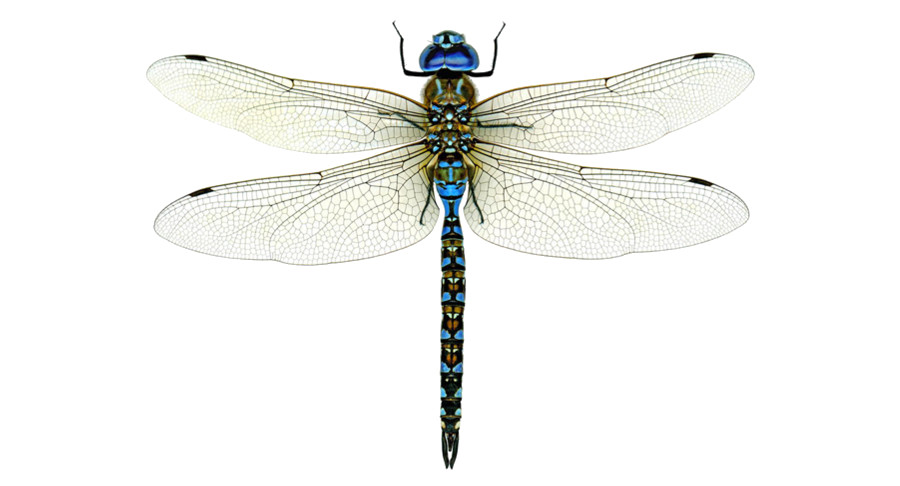
\includegraphics[width=\linewidth]{dragonfly.jpg}

\vspace{0.25 cm}
wings are not limbs
\end{center}

\column{0.35\linewidth}
\begin{center}
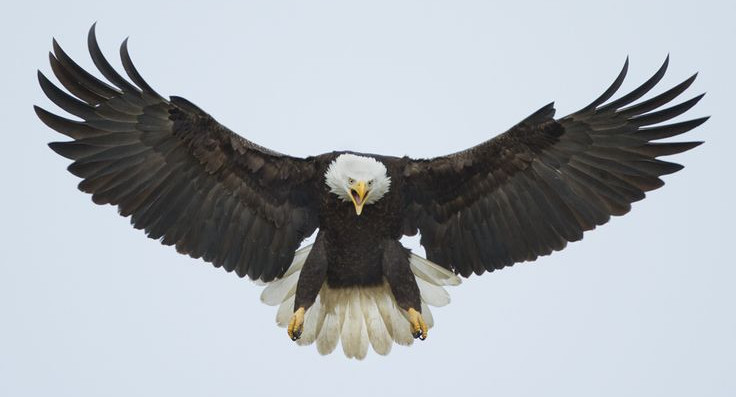
\includegraphics[width=\linewidth]{bird.jpg}

\vspace{0.25 cm}
wings are arms
\end{center}

\column{0.35\linewidth}
\begin{center}
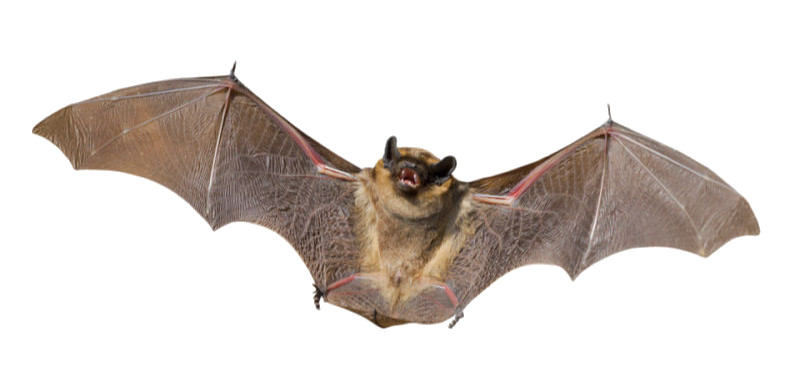
\includegraphics[width=\linewidth]{bat.jpg}

\vspace{0.25 cm}
wings are hands
\end{center}
\end{columns}
\end{frame}

\begin{frame}{Feature comparison: ROOT and Parquet}
\vspace{0.5 cm}
\begin{columns}[t]
\column{0.5\linewidth}
{\large \underline{ROOT}}

\begin{itemize}
\item Store individual C++ objects rowwise in TDirectories and large collections of C++ objects (or simple tables) rowwise or columnar in TTrees.
\item Can write many times, like HDF5 or a database, but most users write once.
\item \textcolor{darkorange}{Selective reading of columns (same).}
\item \textcolor{darkorange}{Cluster/basket structure (same).}
\item Plain encodings, one level of depth (after which the encoding is rowwise).
\item Compression codecs: gzip, lz4, lzma, \textcolor{gray}{zstd (in consideration)}
\end{itemize}

\column{0.5\linewidth}
{\large \underline{Parquet}}

\begin{itemize}
\item Only store large collections of language-independent, columnar objects. No handling of solitary or rowwise objects.
\item Write once, producing an immutable artifact.
\item \textcolor{darkorange}{Selective reading of columns (same).}
\item \textcolor{darkorange}{Row group/page structure (same).}
\item Highly packed encodings, any level of depth (logarithmic scaling with depth).
\item Compression codecs: snappy, gzip, lzo, brotli, \textcolor{gray}{lz4, zstd (version 2.3.2)}
\end{itemize}
\end{columns}
\end{frame}

\begin{frame}{Implementation comparision: ROOT and Parquet (1)}
\vspace{0.5 cm}
\begin{columns}[t]
\column{0.5\linewidth}
{\large \underline{ROOT}}

\begin{itemize}
\item First object in the file is a header providing metadata and seek points to other data structures in the file.

\item Header must be rewritten during file-writing to point to new objects.

\item Failure is partially recoverable, but the writing is non-sequential.

\item Facilitates use of ROOT as a database.
\end{itemize}

\column{0.5\linewidth}
{\large \underline{Parquet}}

\begin{itemize}
\item Last 4 bytes specify a footer size, immediately before that is a footer with metadata and seek points.

\item Objects are written sequentially and only pointed to at the end.

\item Failure invalidates the whole file, but writing is sequential.

\item Parquet is intended to be write-once.
\end{itemize}
\end{columns}
\end{frame}

\begin{frame}{Implementation comparision: ROOT and Parquet (2)}
\vspace{0.5 cm}
\begin{columns}[t]
\column{0.5\linewidth}
{\large \underline{ROOT}}

\begin{itemize}
\item Data structures for metadata are specified by streamers, which relate bytes on disk to fields in C++ class.

\item Data in the large collections (if not simple tables) are specified by the same streamers.

\item Streamer mechanism has built-in schema evolution.

\item Data types are C++ types.
\end{itemize}

\column{0.5\linewidth}
{\large \underline{Parquet}}

\begin{itemize}
\item Reuses Thrift, a rowwise data specification, for the metadata, inheriting its schema evolution.

\item Separately specifies a physical schema (how the data are represented in terms of simple types) and logical schema (mapping onto an existing type system). Data types are independent of any programming language.
\end{itemize}
\end{columns}
\end{frame}

\begin{frame}{Implementation comparision: ROOT and Parquet (3)}
\vspace{0.5 cm}
\begin{columns}
\column{0.5\linewidth}
{\large \underline{ROOT}}

\begin{itemize}
\item Variable-sized data enabled by two arrays: contiguous data content and pointers to the start of each object.

\item Permits random access by entry index.
\end{itemize}

\column{0.5\linewidth}
{\large \underline{Parquet}}

\begin{itemize}
\item Contiguous data array accompanied by two more arrays:
\begin{itemize}
\item definition levels: integers indicating depth of first {\tt\small null} in data; maximum for non-null data.
\item repetition levels: integers indicating depth of continuing sub-list, e.g.\ {\tt\small 0} means new top-level list.
\end{itemize}

\item Definition levels required for non- nullable data, to encode empty lists.

\item Schema depth fixes maximum definition/repetition values, and therefore number of bits in their representations.
\end{itemize}
\end{columns}
\end{frame}

\begin{frame}{Implementation comparision: ROOT and Parquet (4)}
\vspace{0.5 cm}
\begin{columns}
\column{0.5\linewidth}
{\large \underline{ROOT}}

\begin{itemize}
\item Data are simply encoded, by streamers or as basic C++ types (e.g.\ {\tt\small Char\_t, Int64\_t, float, double}).
\end{itemize}

\column{0.5\linewidth}
{\large \underline{Parquet}}

\begin{itemize}
\item Integers and booleans with known maximum are packed into the fewest possible bits.

\item Other integers are encoded in variable-width formats, e.g.\ 1~byte up to 127, 2~bytes up to 16511, zig-zagging for signed integers.

\item Switches between run length encoding and bit-packing dynamically.

\item Optional ``dictionary encoding,'' which replaces data with a dictionary of unique values and indexes into that dictionary (variable-width encoded).
\end{itemize}
\end{columns}
\end{frame}

\begin{frame}{Implementation comparision: ROOT and Parquet (5)}
\vspace{0.5 cm}
\begin{columns}
\column{0.5\linewidth}
{\large \underline{ROOT}}

\begin{itemize}
\item Granular unit of reading/decompression is a basket, which may be anywhere in the file (located by TKey).

\item Basket boundaries may line up in clusters (controlled by autoflush). Clusters are a convenient unit of parallelization.
\end{itemize}

\column{0.5\linewidth}
{\large \underline{Parquet}}

\begin{itemize}
\item Footer specifies row groups, which are like ROOT's clusters, but enforced. Row groups are the granular unit of parallelization (usually tuned to HDFS block size).

\item Data for one column of a row group are split into pages, the granular unit of reading/decompression.

\item Pages of a column are contiguous, always effectively like ROOT's ``{\tt\small SortBasketsByBranch}.''
\end{itemize}
\end{columns}
\end{frame}

\begin{frame}{}
\vspace{0.5 cm}
\begin{center}
\Huge \textcolor{darkblue}{File size comparisons}
\end{center}
\end{frame}

\begin{frame}{Parameters of the test}
\vspace{0.35 cm}
\begin{description}
\item[Datasets:] 13 different physics samples in CMS NanoAOD.

\vspace{0.2 cm}
Non-trivial structure: variable length lists of numbers, but no objects.

\item[ROOT:] 6.12/06 (latest release)

\begin{itemize}
\item Cluster sizes: 200, 1000, 5000, 20\,000, 100\,000 events
\item Basket size: 32\,000 bytes (1~basket per cluster in all but the largest)
\item Freshly regenerated files in this ROOT version: {\tt\small GetItem} from CMS originals and {\tt\small Fill} into the datasets used in this study.
\end{itemize}

\item[Parquet:] parquet-cpp-1.3.1 inside pyarrow-0.8.0 (latest release)

\begin{itemize}
\item Parquet files generated from ROOT via uproot: fully controlling array size so that each Parquet row group is identical to a ROOT cluster, each page is a basket.
\item Parquet files contain the complete semantic information of the original, with a physical schema generated from the TTree's branch structure.
\end{itemize}
\end{description}
\end{frame}

\begin{frame}{Uncompressed Parquet is smaller than ROOT, but gzip is the same}
\vspace{-0.1 cm}
\begin{columns}
\column{0.26\linewidth}
\begin{center}
ROOT uncompressed

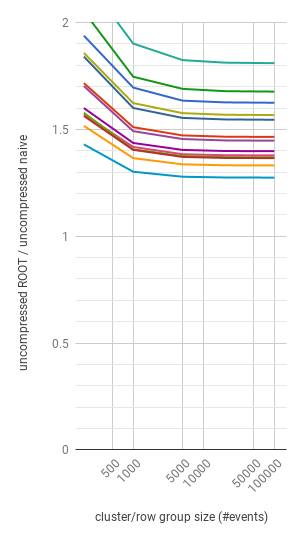
\includegraphics[width=\linewidth]{root-none.png}
\end{center}
\column{0.26\linewidth}
\begin{center}
Parquet uncompressed

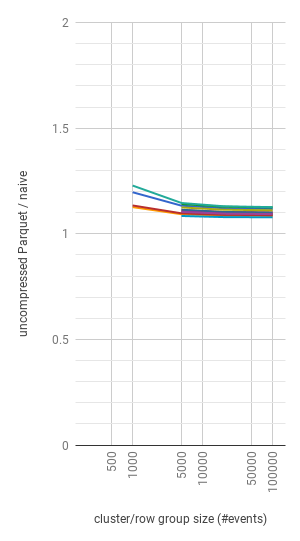
\includegraphics[width=\linewidth]{parquet-none.png}
\end{center}
\column{0.26\linewidth}
\begin{center}
ROOT gzip

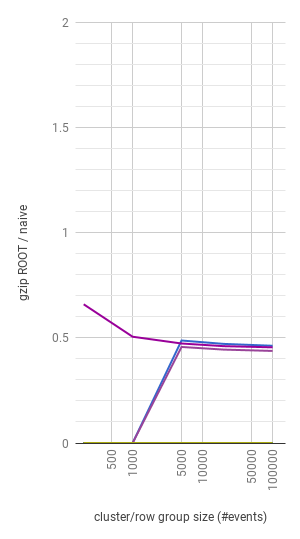
\includegraphics[width=\linewidth]{root-gzip.png}
\end{center}
\column{0.26\linewidth}
\begin{center}
Parquet gzip

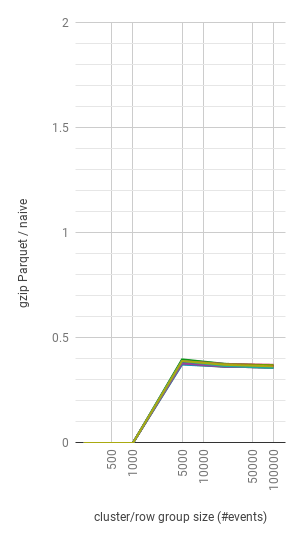
\includegraphics[width=\linewidth]{parquet-gzip.png}
\end{center}
\end{columns}

\vspace{0.25 cm}
Ensemble of 13 physics types vs.\ cluster size/row group size.
\end{frame}

\begin{frame}{But Parquet's dictionary encoding is close to ROOT's full gzip}
\begin{columns}
\column{0.26\linewidth}
\begin{center}
\mbox{\hspace{3 cm}}
ROOT gzip

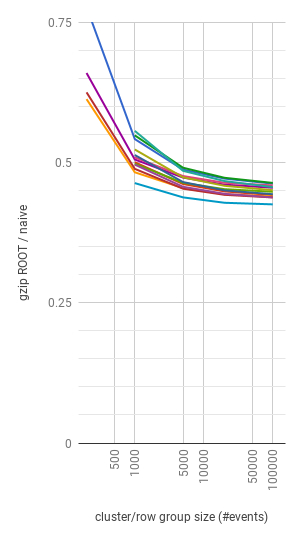
\includegraphics[width=\linewidth]{root-gzip-2.png}
\end{center}
\column{0.26\linewidth}
\begin{center}
\mbox{\hspace{3 cm}}
ROOT lzma

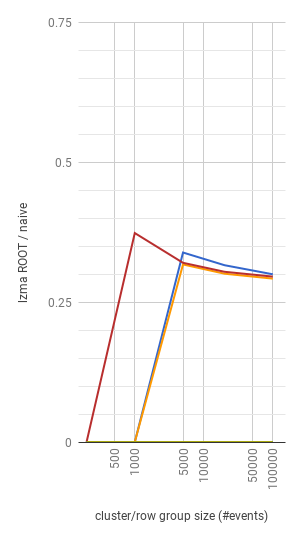
\includegraphics[width=\linewidth]{root-lzma.png}
\end{center}
\column{0.26\linewidth}
\begin{center}
\mbox{\hspace{3 cm}}
Parquet gzip

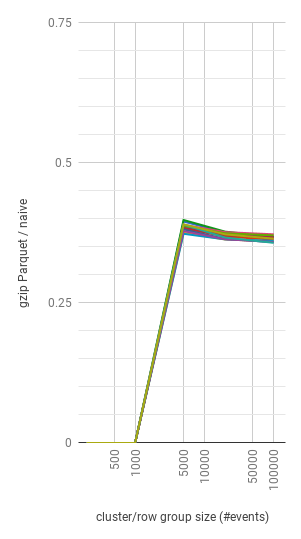
\includegraphics[width=\linewidth]{parquet-gzip-2.png}
\end{center}
\column{0.26\linewidth}
\begin{center}
Parquet uncompressed
with dict encoding

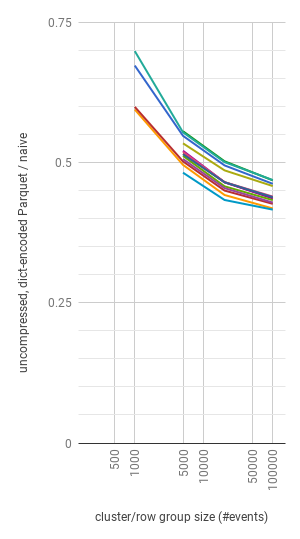
\includegraphics[width=\linewidth]{parquet-dict.png}
\end{center}
\end{columns}
\end{frame}

\begin{frame}{Tabular comparison}
\vspace{0.5 cm}
Highest cluster/row group (100\,000 events), total file size (sum of 13 physics types):

\begin{center}
\begin{tabular}{r c c | c c}
                    & \multicolumn{2}{c}{all branches} & \multicolumn{2}{c}{without trigger} \\
                    & ROOT & Parquet & ROOT & Parquet \\\hline
uncompressed        & \ldots & \ldots & \ldots & \ldots \\
dictionary encoding & & \ldots & & \ldots \\
lz4                 & \ldots & & \ldots & \\
gzip                & \ldots & \ldots & \ldots & \ldots \\
lzma                & \ldots & & \ldots & \\
\end{tabular}
\end{center}

$601+21$ of NanoAOD's $955$ branches are booleans named {\tt\small HLT\_*} or {\tt\small Flag\_*}, which unnecessarily increase the uncompressed ROOT size.
\end{frame}




\end{document}
